\documentclass[]{article}

\usepackage{listings}
\usepackage{color}
\usepackage{amsmath}
\usepackage{graphicx}
\usepackage{float}
\usepackage[title]{appendix}
\usepackage[ansiapaper, portrait, margin=1.5in]{geometry}
\usepackage{hyperref}

\usepackage{caption}
\usepackage{subcaption}

\usepackage[backend=biber]{biblatex}
\addbibresource{comp-physics-project-may13.bib}

\definecolor{dkgreen}{rgb}{0,0.6,0}
\definecolor{gray}{rgb}{0.5,0.5,0.5}
\definecolor{mauve}{rgb}{0.58,0,0.82}




\hypersetup{
	colorlinks=false %set true if you want colored links
	linktoc=all,     %set to all if you want both sections and subsections linked
	linkcolor=blue,  %choose some color if you want links to stand out
}
\hypersetup{hidelinks}

\lstset{frame=tb,
	language=Python,
	aboveskip=3mm,
	belowskip=3mm,
	showstringspaces=false,
	columns=flexible,
	basicstyle={\small\ttfamily},
	numbers=none,
	numberstyle=\tiny\color{gray},
	keywordstyle=\color{blue},
	commentstyle=\color{dkgreen},
	stringstyle=\color{mauve},
	breaklines=true,
	breakatwhitespace=true,
	tabsize=3
}

%opening
\title{May 14th Weekly Report}
\author{Erik Bigwood}

\begin{document}

\maketitle

\begin{abstract}
In total, this week I have extended my work to analyze the physics of two same-charged particles in a harmonic potential. Adopting the exact form of the Lagrangian used to generate the synthetic dataset provided a robust fit to the data, converging well under a suitable loss function ($L^2$ norm). This method extended partially to cases with the sampling window -- large displacements blocked convergence for $\alpha$ but converged well for $k$, and a narrow window around one of the two fixed points converged exceedingly well.

Adding complexity to the Lagrangian by considering a polynomial in $q_0$ and $q_1$ had somewhat more mixed results. Fitting around the origin and in a wide window around a fixed point largely succeeded, but fitting a narrow window around a fixed point and then extending to validate this fit over a wide region failed  just about everywhere except in the narrow training window.

To facilitate these more computationally demanding experiments, I have made a couple of improvements to the core algorithm by further leveraging torch.func.vmap.
\end{abstract}

\tableofcontents
\newpage

\section{Two particles in a harmonic potential with Coulomb repulsion, exact Lagrangian}
\subsection{Basic results}

\paragraph{Code setup}
Here I've created and system with two particles in a 1D harmonic potential (strength $k$) \cite{Taylor2005} with a Coulomb potential \cite{Griffiths2013} between them ($\alpha=charge_0\cdot charge_1$), both masses set to 1. As the dimension of the phase space here is twice as large as the 1D system, and in anticipation of future expansions, I've rewritten the phase-space sampling as a large number of random points instead of a grid.

\begin{lstlisting}
	q0_min, q0_max, q1_min, q1_max, = -1, 1, -1, 1
	Q0 = (q0_max - q0_min)*(torch.rand(n_points)) + q0_min
	Q1 =  (q1_max - q1_min)*(torch.rand(n_points)) + q1_min
	
	qdot_min, qdot_max = -1, 1
	qdot_sampling = (qdot_max - qdot_min)*(torch.rand([2,n_points])) + qdot_min
	QD0 = qdot_sampling[0,:]
	QD1 = qdot_sampling[1,:]
\end{lstlisting}

Package these into array objects to be passed to later functions:

\begin{lstlisting}
	Qv = torch.zeros(n_points,2)
	Qv[:,0] = Q0
	Qv[:,1] = Q1
	
	QDv = torch.zeros(n_points,2)
	QDv[:,0] = QD0
	QDv[:,1] = QD1
\end{lstlisting}

Then calculate the predicted $\ddot{q}$  values in a single call:

\begin{lstlisting}
	out = QDDv(Qv,QDv,m,k,alpha)
	outmag = (out[:,0]**2 + out[:,1]**2)**.5
\end{lstlisting}

\subsubsection{Results}
In Fig. \ref{fig:quiver-sampling}, I've included a quiver plot of the unit vectors $\ddot{q}/|\ddot{q}|$ and a scatter plot colored by $|\ddot{q}|$. Since the band where $|q_0-q_1|$ is small produces very large generalized forces, I've removed any points in it to reduce numerical instability later in the fitting algorithm. These points produce a much larger contribution to the loss, they contribute to extremely large gradients along the $\alpha$ axis of parameter space that largely wash out the contribution from $k$ and delay convergence under gradient descent.

In the quiver plot, we see the exluded band of extreme $\ddot{q}$ as well as a pair of points where $\ddot{q}$ goes to zero. These are the points in $(q_0,q_1)$ configuration space such that the harmonic and Coulomb forces balance and the particles are not accelerated.  Away from this region, $\ddot{q}$ becomes dominated by the the harmonic potential.
\begin{figure}[H]
	\caption{Quiver and scatter plots of sampled points and associated $\ddot{q}$}
	\centering
	\includegraphics[scale=0.35]{2D-sampling.png}
	\label{fig:quiver-sampling}
\end{figure}

Now calculating the loss landscape around the true ($k$, $\alpha$) parameters, we see a deep well of low loss in Fig. \ref{fig:loss-landscape}, with the caveat of mismatched gradients between $k$ and $\alpha$ directions.

\begin{figure}[H]
	\caption{Loss landscape vs. ($k$, $\alpha$)}
	\centering
	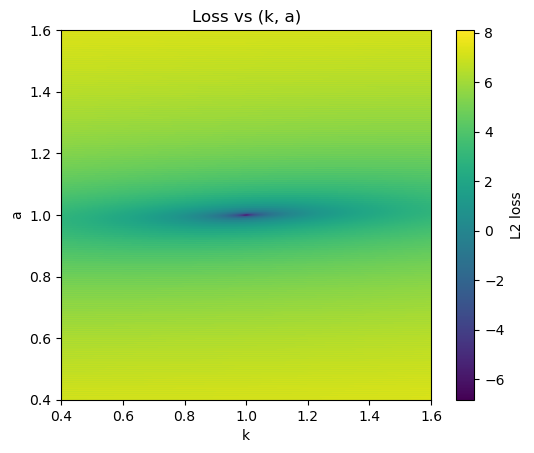
\includegraphics[scale=0.70]{loss-landscape.png}
	\label{fig:loss-landscape}
\end{figure}

Performing gradient descent on this landscape leads to convergence on the small valley of low loss as expected, but this convergence is slow compared to the 1D case due to the mismatch of gradient magnitude between the $k$ and $\alpha$ directions. See Fig. \ref{fig:gradient-descent-paths}. In general, gradient descent in this type of situation will tend to optimize the variable with the larger gradient first (and quickly), and then slowly optimize the other. In future updates I will try using more modern optimizers like 'Adam'\cite{Kingma2014} or 'AdaGrad'\cite{Duchi2011}  that purport to perform better in these situations.

\begin{figure}[H]
	\caption{Gradient descent on loss landscape vs. ($k$, $\alpha$)}
	\centering
	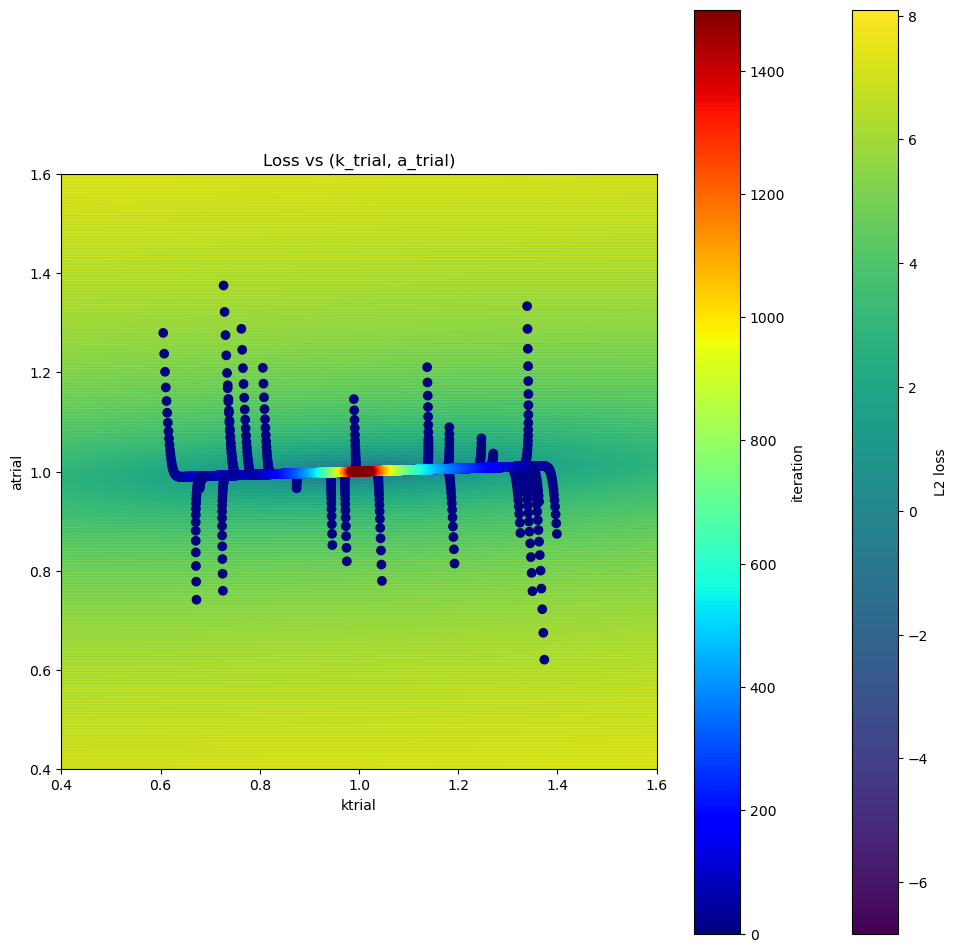
\includegraphics[scale=0.60]{gradient-descent-paths.png}
	\label{fig:gradient-descent-paths}
\end{figure}

In Fig. \ref{fig:convergence}, I've plotted both the loss (\ref{subfig:convergence-loss}) and parameter fit (\ref{subfig:convergence-ratio}). As expected, loss monotonically decreases and does not appear to saturate (running further iterations would likely decrease loss even further). For the parameter fit, I've plotted the ratio of the experimental $(l/\alpha)$ and the true $k/\alpha$, showing clean convergence to the true parameters.

\subsection{Changing sampling areas}
\subsubsection{Far from the origin}
Not all experimental situations will have such clear coverage over regions of phase space with strong influence from interactions. Displacing the sampled region of phase space away from makes the sampled $\ddot{q}$ dominated by the harmonic potential and reduces the gradient in the $\alpha$ direction.

This displacement increases the magnitude of the $k$ gradient and dramatically reduces the magnitude of the $\alpha$ gradient, as expected by the scaling of the harmonic and Coulomb potentials under displacement. Fig. \ref{fig:loss-landscape-father-away} contains a plot of the loss landscape, which notably has some unexpected roughness that persists over large ranges of the number of sampled phase space points.

\begin{figure}[H]
	\caption{Loss landscape vs. ($k$, $\alpha$), sampling displaced from the origin}
	\centering
	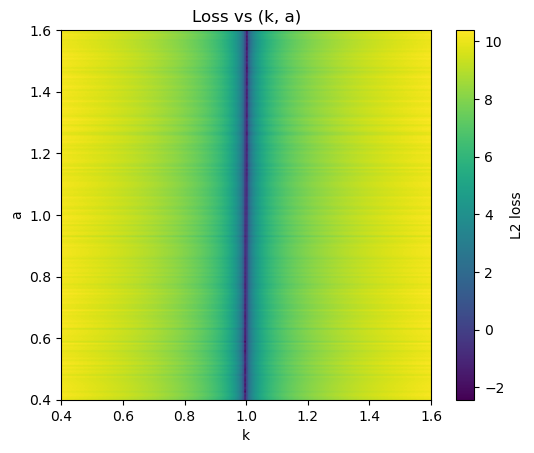
\includegraphics[scale=0.70]{loss-landscape-farther-away.png}
	\label{fig:loss-landscape-father-away}
\end{figure}

Performing gradient descent on this displaced dataset is far less successful -- only $k$ converges to the correct value in Fig. \ref{fig:gradient-descent-paths-father-away}. $\alpha$ only converges a very small amount due to the mismatch between gradient magnitudes, addressing this would require tuning the learning rate to compensate for this difference and reducing the landscape roughness. I tried tuning the algorithm to dramatically increase the learning rate as the loss value decreases, but this only resulted the system getting trapped in local minima caused by the roughness. Fig. \ref{fig:convergence-farther-away} contains plots of the loss (\ref{subfig:convergence-loss-father-away}) and $k/\alpha$ (\ref{subfig:convergence-ratio-farther-away}) performance trends, further indicating the optimizer getting trapped in local minima along the $k=1$ line.

\begin{figure}[H]
	\caption{Gradient descent on loss landscape vs. ($k$, $\alpha$), displaced from the origin}
	\centering
	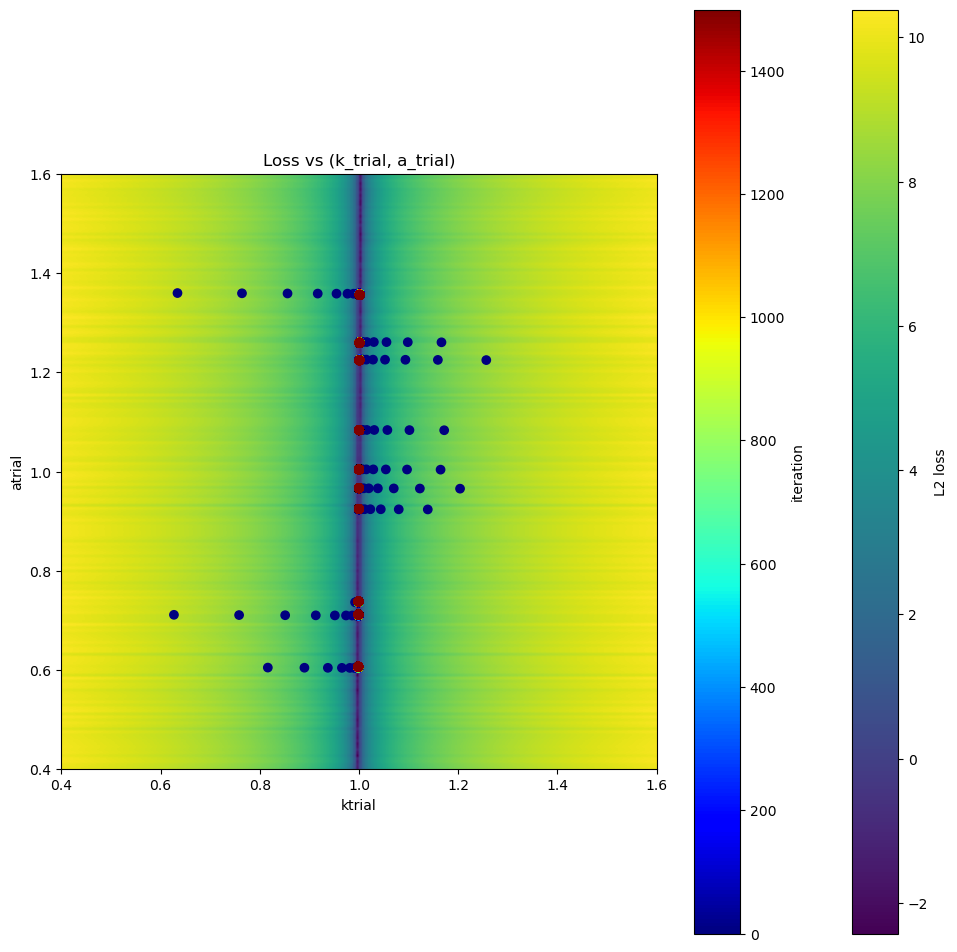
\includegraphics[scale=0.60]{gradient-descent-paths-farther-away.png}
	\label{fig:gradient-descent-paths-father-away}
\end{figure}

\subsubsection{Near a fixed point}
Near one of the fixed points where the harmonic and Coulomb forces balance, the story changes a bit. Fig. \ref{fig:2D-sampling-fixed-point} shows the sampled points and associated $\ddot{q}$. The loss landscape (Fig. \ref{fig:loss-landscape-fixed-point}) shows a strong loss well, but some additional roughness that appears to be worse with fewer sampled points. 

\begin{figure}[H]
	\caption{Loss landscape vs. ($k$, $\alpha$), sampling near a fixed point}
	\centering
	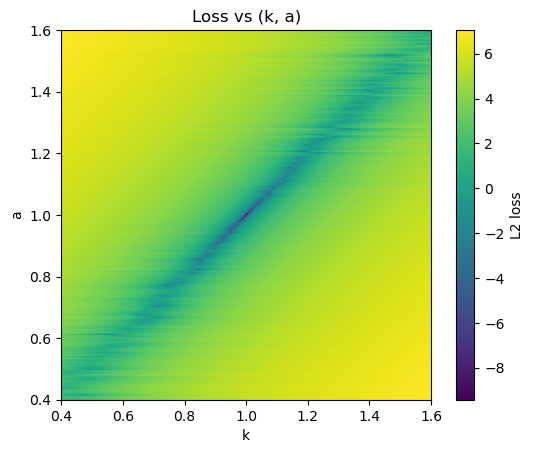
\includegraphics[scale=0.70]{loss-landscape-fixed-point.png}
	\label{fig:loss-landscape-fixed-point}
\end{figure}

This roughness does not preclude proper convergence, as gradient descent performs reasonably well. In this setup we still see that the magnitude of the gradients are mismatched, but this time the system converges to the $k=\alpha$ line and then slowly optimizes towards the true parameters. The performance parameters are plotted in Fig. \ref{fig:convergence-fixed-point}, with both loss (\ref{subfig:convergence-loss-fixed-point}) and $k/\alpha$ (\ref{subfig:convergence-ratio-fixed-point}) indicating extremely robust convergence to the true solution. As seen before, this optimization proceeds in two phases -- first, the system falls onto the $k=\alpha$ line, and then falls towards the low loss point at the true parameter values.

\begin{figure}[H]
	\caption{Gradient descent on loss landscape vs. ($k$, $\alpha$), near a fixed point}
	\centering
	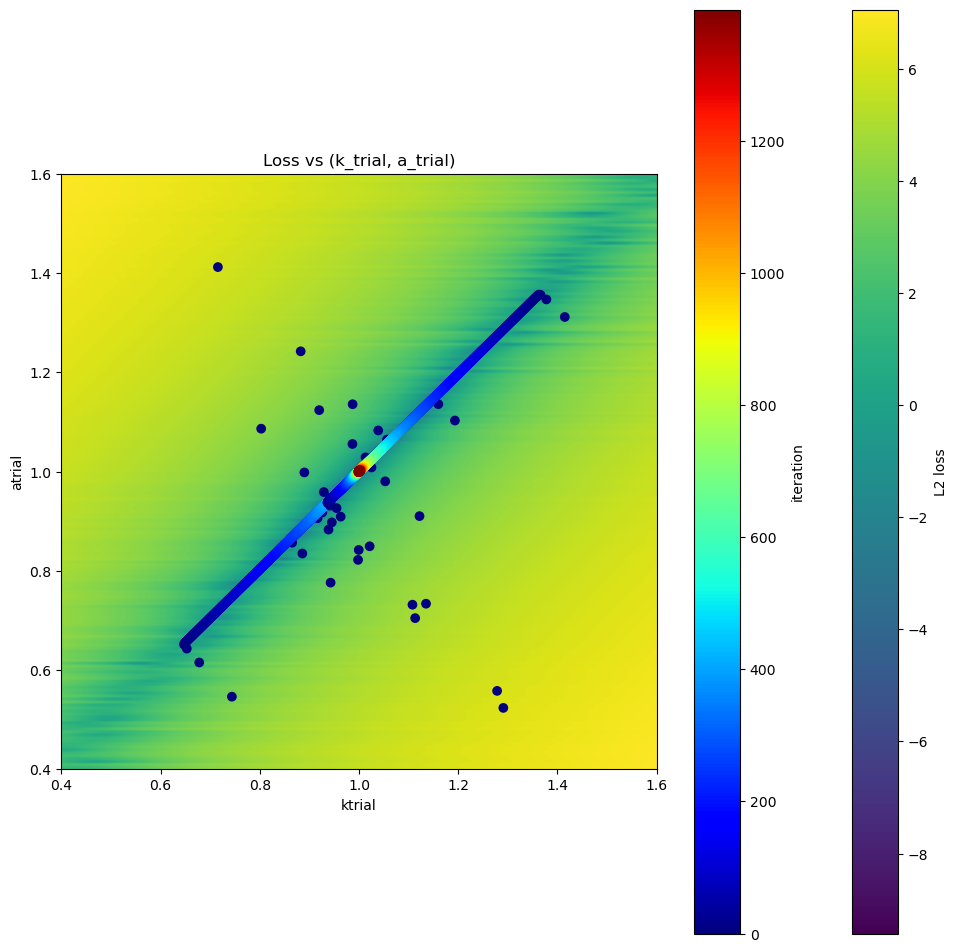
\includegraphics[scale=0.60]{gradient-descent-paths-fixed-point.png}
	\label{fig:gradient-descent-paths-fixed-point}
\end{figure}

Interestingly, zooming the sampling far into this fixed point region reduces the loss landscape roughness (Fig. \ref{fig:loss-landscape-fixed-point-close}) by a large degree, and deepens the low-loss valley to the lowest loss value $(\approx10^{-25})$ seen in any run so far.

Comparing the quiver plots  in Fig. \ref{fig:sampling-fixed-point} for the zoomed-out (sampling region $0.1$ units wide, \ref{subfig:sampling-fixed-point}) and zoomed-in (sampling region $0.0002$ units wide, \ref{subfig:sampling-fixed-point-close}) sampling around the fixed points seems to show very similar behavior across these different scales. In further updates I may explore this further, with special attention on any possible mapping to other physical systems, and possible scaling symmetries.



\begin{figure}[H]
	\caption{Loss landscape vs. ($k$, $\alpha$), sampling zoomed in on a fixed point}
	\centering
	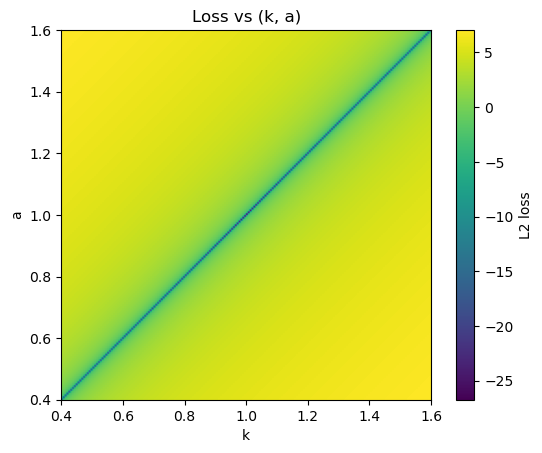
\includegraphics[scale=0.70]{loss-landscape-fixed-point-close.png}
	\label{fig:loss-landscape-fixed-point-close}
\end{figure}

\section{Two particles in a harmonic potential with Coulomb repulsion, polynomial Lagrangian}
\subsection{Problem setup}
As before, I generate a synthetic dataset from the exact Lagrangian with known parameters, then disregard those known parameters for fitting. Here I move to a more complicated Lagrangian that is a polynomial in powers of products of the coordinates $q$ and quadratic in $\dot{q}$ as follows:


\begin{equation}
	\mathcal{L} = \frac{1}{2} \dot{q}^2 + \sum_{m=0}^{n_{particles}} \sum_{n=0}^{n_{particles}} \Bigg[\sum_{i=1}^{N} \sum_{j=1}^{N} c_{m,n,i,j} q_m^i q_n^j\Bigg]
\end{equation}

Where $q_m$ is the $m$-th component of $q$ (in this 1D case, the value of $q$ for the $m$-th particle) and $c_{m,n,i,j}$ is the parameter tensor/weight for the $(m,n,i,j)$-th term in this polynomial. For implementation in this 1D, 2 particle system, the code actually discards the initial double sum over $(m,n)$ in favor of summing over the three configurations $(m,n)$ = $(0,0)$, $(0,1)$, and $(1,1)$ as the $(0,1)$ case is equivalent to $(1,0)$. This then reduces to the following where $\mathcal{M}$ is the set containing those three cases:

\begin{equation}
	\mathcal{L} = \frac{1}{2} \dot{q}^2 + \sum_{(m,n)\in\mathcal{M}}  \Bigg[\sum_{i=1}^{N} \sum_{j=1}^{N} c_{m,n,i,j} q_m^i q_n^j\Bigg]
\end{equation}

Unfortunately, this becomes rather large and compute-intensive quickly as the number of terms $N$ is increased. So far I have only explored out to $N=8$ on an nVidia T4 GPU provided by Google Colab. Training this Lagrangian presents additional challenges relative to training a Lagrangian with the same structure as the true one, especially with interactions like this Coulomb potential. The Coulomb potential term $\alpha(\frac{1}{|q_0-q_1|})$ expands as a binomial series\cite{Binomial}. Taking the $q_0=1$ case, this  becomes (within a suitable radius of convergence $|q_1|<1$):

\begin{equation}
	\Big|\frac{1}{q_0-q_1}\Big| \to \Big| (1-q_1)^{-1}\Big| = \Big|\sum_{k=0}^{\infty} \frac{(1)_k}{k!}q_1^k\Big| = \Big|1 + q_1 + q_1^2 + q_1^3 + ...\Big|
\end{equation}

This expression contains terms of arbitrarily high order, so no finite polynomial will perfectly fit this system. Instead, an approximation for the true Lagrangian is optimized by the algorithm, minimizing the prediction loss at each sample point.

\subsection{Results}
\paragraph{First runs}
Take as a first example a training run on this polynomial Lagrangian from a dataset with $m=1$, $k=4$, and $\alpha=1$. The loss history/profile is shown in Fig. \ref{fig:poly-loss-training-1}, and converges acceptable, although dramatically slower than the exact form Lagrangian due to the vastly increased number of parameters.

This training resulted in (Fig. \ref{fig:poly-fit-1}) a learned Lagrangian that fits the dataset reasonably well -- it has fixed representing the equilibra from the harmonic and Coulomb forces balancing, and matches the rough overall trends. There are, however, distinct errors in this run, such as fit arrows pointing outwards at the borders of the sampled region instead of in as in the dataset. 

\begin{figure}[H]
	\caption{Sampled points and trained polynomial Lagrangian results, run 1}
	\centering
	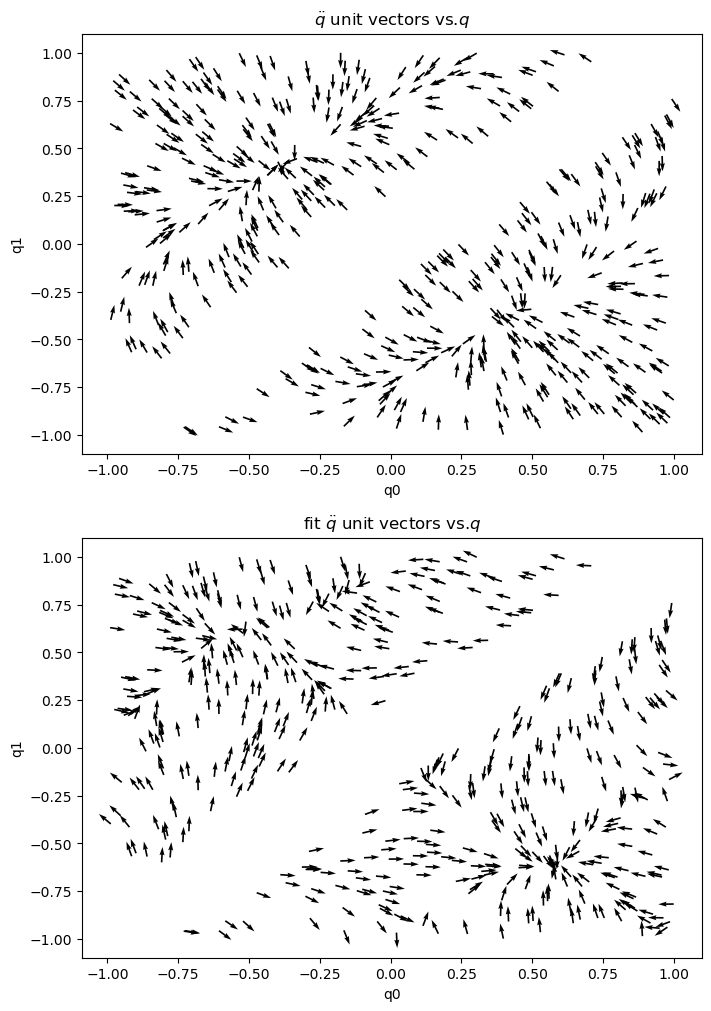
\includegraphics[scale=0.60]{poly-fit-1.png}
	\label{fig:poly-fit-1}
\end{figure}

The learned parameters can be visualized via a density plot, where each region corresponds to a specific term in the polynomial. In Fig. \ref{fig:poly-coupling-parameters-1}, I've plotted the polynomial coefficients for only the coupling terms $q_0^i \cdot q_1^j$. We see approximate symmetry across the $i=j$ diagonal, and in general runs tend to converge to a symmetric matrix, as we would expect given the coupling term's symmetry in the arguments.

\begin{figure}[H]
	\caption{Polynomial coupling term coefficients, run 1}
	\centering
	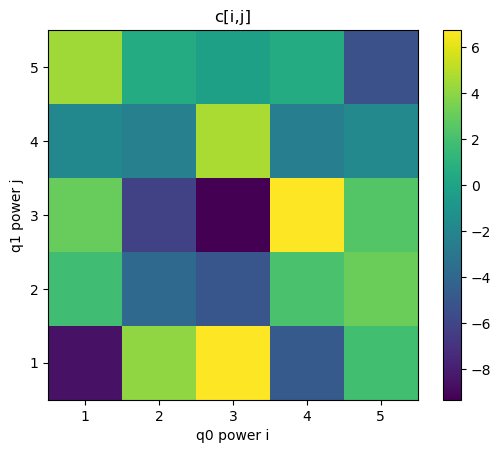
\includegraphics[scale=0.60]{poly-coupling-parameters-1.png}
	\label{fig:poly-coupling-parameters-1}
\end{figure}

\paragraph{Alternate form}
The previous parameter object $c_{m,n,i,j}$ is a $(3\times n_{powers} \times n_{powers})$ element tensor containing a large number of duplicate parameters in the $(m=n)$ slices. To reduce this redundancy and simplify the fitting to just the coupling terms, I define a new (but related) Lagrangian retaining the original values for $m$ and $k$ :
\begin{equation}
	\mathcal{L} = \frac{1}{2} \dot{q}^2 - \frac{1}{2}k q^2 - \Bigg[\sum_{i=1}^{N} \sum_{j=1}^{N} c_{i,j} q_0^i q_1^j\Bigg]
\end{equation}
This bracketed term now contains all of the couplings between the particles and only contains $(n_{powers}\times n_{powers})$ elements to optimize, but neglects any higher powers of individual $q_i$ values (to be addressed later). The convergence performance of this version is similar (Fig. \ref{fig:poly-loss-training-2}), though slightly faster per iteration due to the lower number of parameters. This also produces a result with a good qualitative match to the data set (Fig. \ref{fig:poly-fit-2}), but with the same caveats about errors at the boundaries. For this run, I've restricted the sampling to one side of the $q_0=q_1$ line for visual clarity.


\begin{figure}[H]
	\caption{Sampled points and trained polynomial Lagrangian results, run 2}
	\centering
	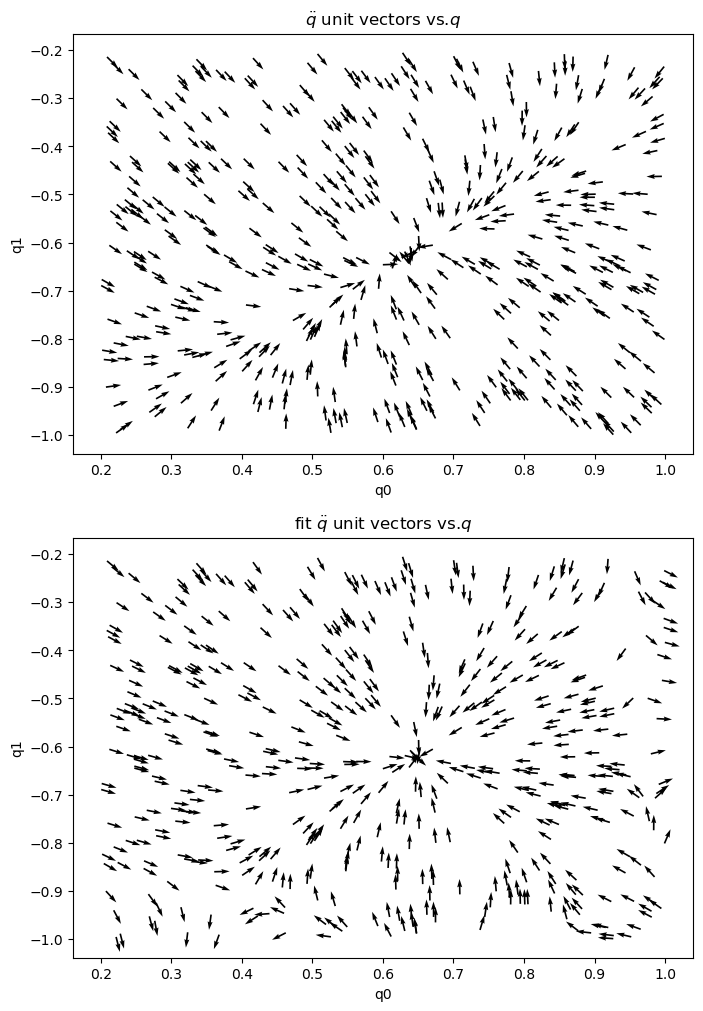
\includegraphics[scale=0.60]{poly-fit-2.png}
	\label{fig:poly-fit-2}
\end{figure}


\begin{figure}[H]
	\caption{Polynomial coupling term coefficients, run 2}
	\centering
	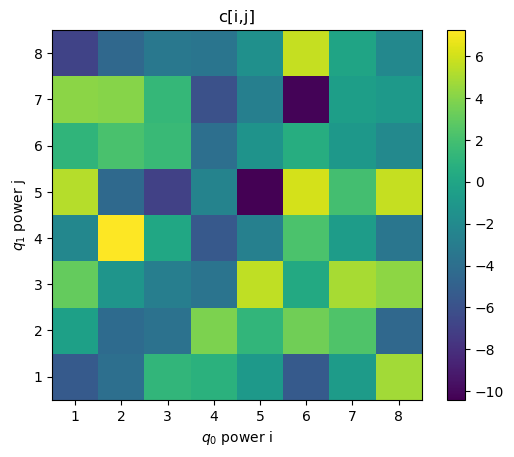
\includegraphics[scale=0.60]{poly-coupling-parameters-2.png}
	\label{fig:poly-coupling-parameters-2}
\end{figure}

The parameters (Fig. \ref{fig:poly-coupling-parameters-2}) learned in this run are not as symmetric as run 1, and interestingly contain much more contribution from the $q_0^8$ terms.


In Fig. \ref{fig:poly-fit-errors-2} I've plotted the absolute errors between dataset $\ddot{q}$ and fit $\ddot{q}$. Near the fixed point (center of frame), the error becomes very small, but the error tends to increase near the boundaries of the sampling region. The error becomes especially large in the upper-left region where the separation between the charges is smallest -- here the generalized force $\ddot{q}$ blows up and is not fully captured. This is to be expected as we are truncating the true coupling term, and its magnitude becomes very large in this region.

\begin{figure}[H]
	\caption{Sampled points vs. trained polynomial Lagrangian error, run 2}
	\centering
	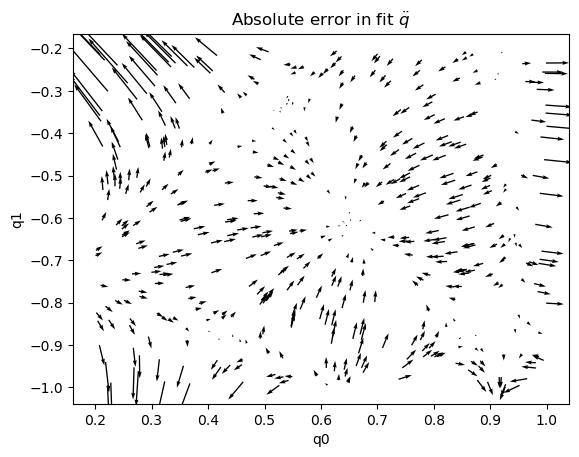
\includegraphics[scale=0.60]{poly-fit-errors-2.png}
	\label{fig:poly-fit-errors-2}
\end{figure}

The relative errors (Fig. \ref{fig:poly-fit-errors-relative-2}) shows different behavior -- there is far less increase for the $q_0\approx q_1$ region in the top left, but the area near (but not exactly at) the fixed point (center) has much more considerable errors. 

\begin{figure}[H]
	\caption{Sampled points and trained polynomial Lagrangian results, run 2}
	\centering
	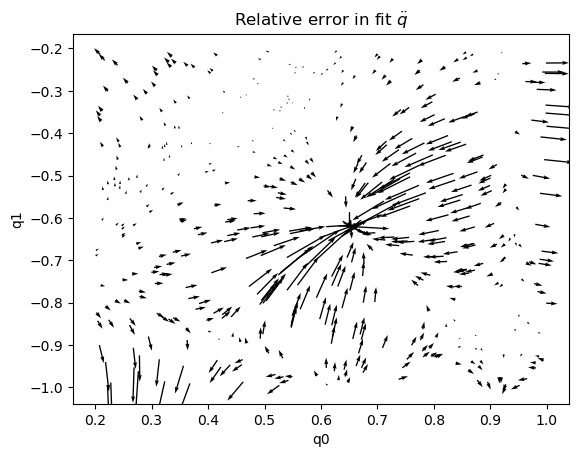
\includegraphics[scale=0.60]{poly-fit-errors-relative-2.png}
	\label{fig:poly-fit-errors-relative-2}
\end{figure}

\subsubsection{Changing the sampling vs. validation window}
I now restrict the sampling points provided to the algorithm to an exceedingly narrow range ($0.0003$ units wide compared to previous windows of $\approx 1$ unit) centered around one of the two fixed points. As mentioned before, at these scales the calculated $\ddot{q}$ unit verctor field appears independent of window size. To explore how well this system can extrapolate to unknown data, I fit the polynomial Lagrangian to this narrow window and then compare its predictions over a wider validation window to the true Lagrangian's results. Notably, this converges much more unsteadily, tending to halt by increasing loss after a long epoch near what appears to be a local minimum (Fig. \ref{fig:poly-loss-training-3}). The results for the fit over the sampling window are at surface level fairly good, although the pinched line from lower left to upper right is rotated to be horizontal in this fit (Fig. \ref{fig:poly-fit-3} ).

\begin{figure}[H]
	\caption{Sampled points and trained polynomial Lagrangian results, run 3 (narrow sampling window)}
	\centering
	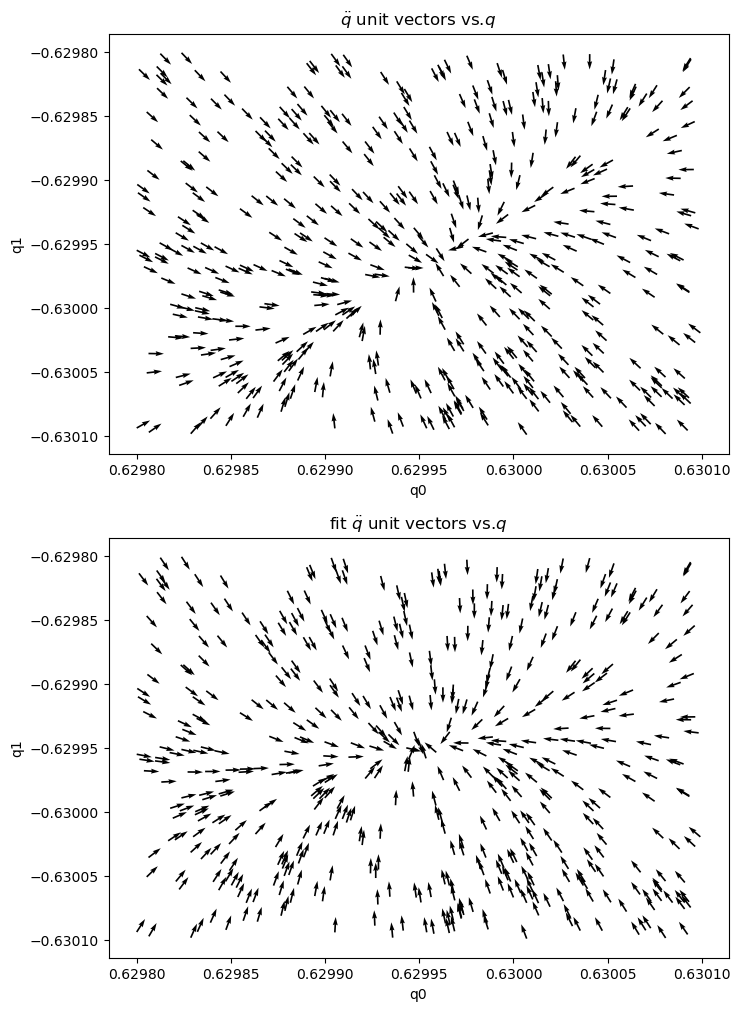
\includegraphics[scale=0.60]{poly-fit-3.png}
	\label{fig:poly-fit-3}
\end{figure}

Expanding the sampling window to a validation window covering both fixed points show how poor this fit truly is -- despite matching well qualitatively on the narrow window, Fig. \ref{fig:poly-fit-3-val} shows that away from the training region, the fit completely fails and produces results that are nothing like the true $\ddot{q}$. Compared to the exact form of the Lagrangian that I fit before, this polynomial appears massively undercontrained when the sampling is inadequate.

\begin{figure}[H]
	\caption{Sampled points and trained polynomial Lagrangian results, run 3 (narrow sampling window)}
	\centering
	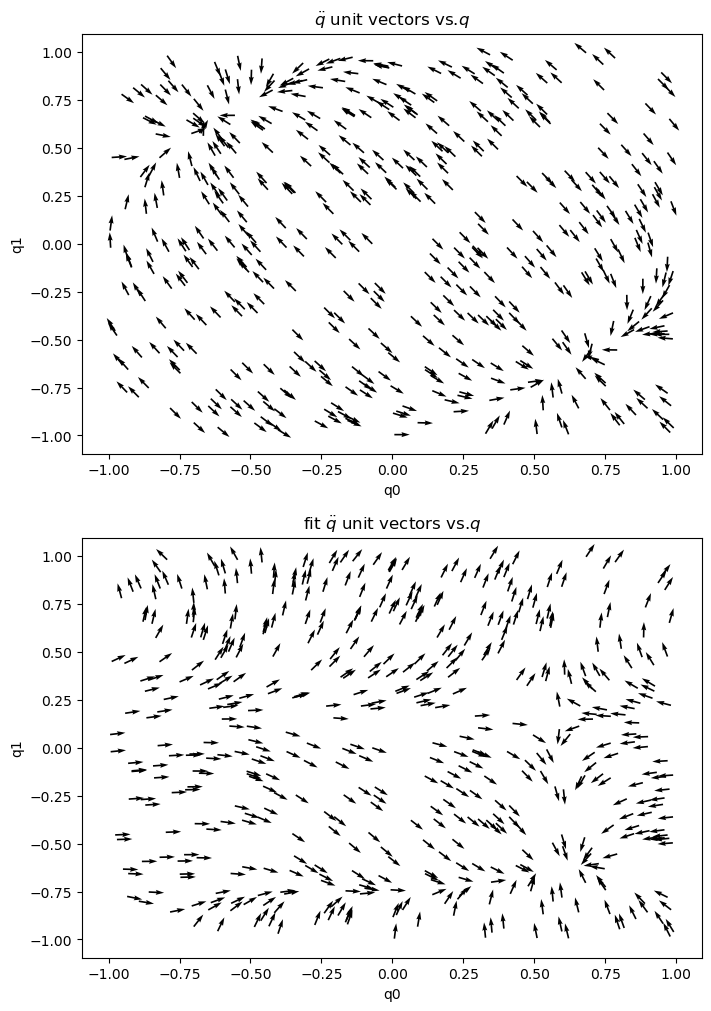
\includegraphics[scale=0.60]{poly-fit-3-val.png}
	\label{fig:poly-fit-3-val}
\end{figure}

This is to some extent the expected behavior -- for this run the parameter tensor $c_{i,j}$ has $9^2=81$ independent elements! I've included the $q_m^i\cdot q_n^0$ terms to allow the system to fit those terms as well. In a future update I will fit the $\ddot{q}$ values for the true Lagrangian to see what kind of form they truly follow in the fixed point regions.




\begin{figure}[H]
	\caption{Polynomial coupling term coefficients, run 2}
	\centering
	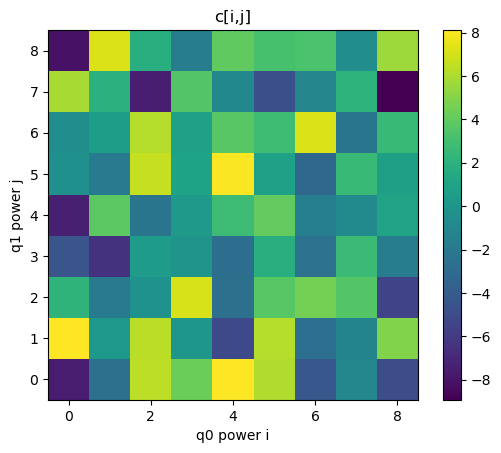
\includegraphics[scale=0.60]{poly-coupling-parameters-3.png}
	\label{fig:poly-coupling-parameters-3}
\end{figure}

\newpage
\section{Algorithm improvements}

\subsection{Plotting loss landscapes}
Previously, to plot an $n\times n$ density plot image, the code iterated via two nested for-loops. This does not take advantage of the full vectorization potention of PyTorch, so I've rewritten it to vectorize along one dimension.

To begin, produce an extended version of the dataset by iteratively concatenating (slow, but workable since the main loss calculation is slow):

\begin{lstlisting}
	n_param_points = 1 #number of copies needed
	
	dataset_expanded = dataset
	for i in range(1,n_param_points):
		dataset_expanded = torch.cat((dataset_expanded,dataset))
\end{lstlisting}

This same process is repeated for the $(q,\dot{q})$ sets and the parameter grid for $\alpha$. Then, redefine the loss function to use the unvectorized function $\ddot{q}$, then wrap it via torch.func.vmap:

\begin{lstlisting}
	def loss(q,qdot,m,k,alpha,dataset):
		test_qdd = QDD(q,qdot,m,k,alpha)
		return torch.sum(( (test_qdd - dataset) )**2 )#/(dataset.size()[0]**2)
	
	lossv = vmap(loss,in_dims=(0,0,None,None,0,0))
\end{lstlisting}

This new function lossv takes in an expanded dataset $(\vec{q},\dot{\vec{q}},m,k,\vec{\alpha})$ (where the vector symbol indicates the expanded dataset), and operates on all elements via PyTorch's built-in vectorization. This produces a dramatic speedup -- for $200\times 200$ pixel images, about 25x.

\subsection{Gradient calculations}
A more effiient formatting for gradient calculations is rewriting the Lagrangian function and all of the higher-order functions as follows:

\begin{lstlisting}
	def L(q,qdot,param):
		return ...
		
	def QDD(q,qdot,param):
		...
		return qdd
	
	def loss(q,qdot,param,dataset):
		return sum( (qdd-dataset)**2 )/dataset.size**2
	
	parameter_gradient = jacrev(loss,argnums=(2))
\end{lstlisting}

Here I'm collecting all of the parameters in one tensor object and passing it, instead of passing individually named parameters like $m$, $k$, $\alpha$, etc. The parameter\_gradient function now returns a tensor of the same size and shape as the parameter tensor containing the gradient of each parameter, so the gradient descent algorithm simplifies to:

\begin{lstlisting}
	parameters = torch.randn([size_0,size_1])
	
	for i in range(n_iterations):
		loss_history[i] = loss(Q,QD,parameters)
		parameters.data -= learning_rate*parameter_gradient(Q,QD,parameters)
\end{lstlisting}

This makes the algorithm more structure-agnostic, simplifying the addition of more complicated Lagrangians like polynomials, neural nets, etc. 



\newpage
\begin{appendices}
\section{Figures}

\subsection{Exact Lagrangian form}
\subsubsection{Basic results}

\begin{figure}[H]
	\caption{Gradient descent performance profile}
	\begin{subfigure}{.5\textwidth}
		\subcaption{Loss vs. iterations}
		\centering
		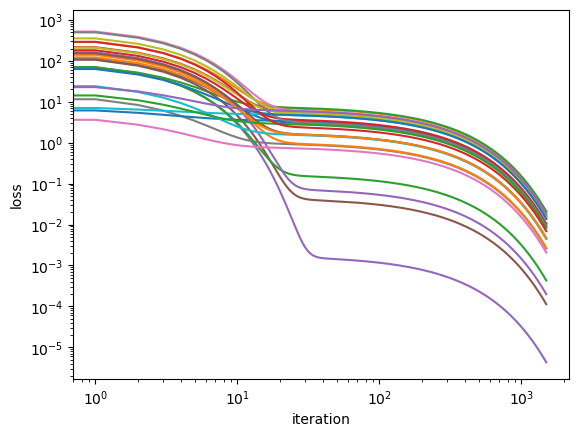
\includegraphics[scale=0.40]{loss-vs-iteration.png}
		\label{subfig:convergence-loss}
	\end{subfigure}
	\begin{subfigure}{.5\textwidth}
		\subcaption{$(k_{exp}/\alpha_{exp})$ $/$ $(k_{true}/\alpha_{true})$ vs. iteration}
		\centering
		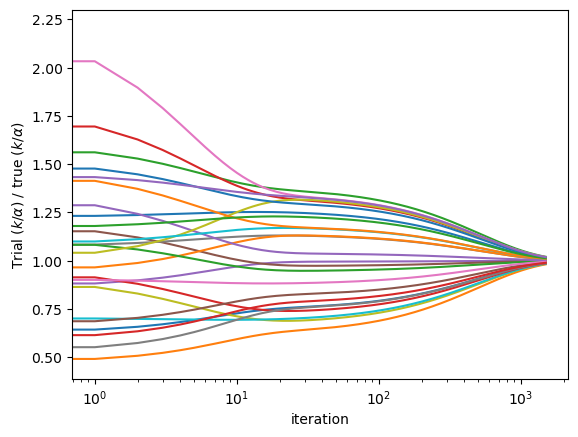
\includegraphics[scale=0.40]{k-a-ratio.png}
		\label{subfig:convergence-ratio}
	\end{subfigure}
	\label{fig:convergence}
\end{figure}

\subsubsection{Sampling far from the origin}

\begin{figure}[H]
	\caption{Sampled points and associated $\ddot{q}$, for $(q_0,q_1)$ displaced from the origin}
	\centering
	\includegraphics[scale=0.40]{2D-sampling-farther-away.png}
	\label{fig:2D-sampling-father-away}
\end{figure}

\begin{figure}[H]
	\caption{Gradient descent performance profile, displaced from the origin}
	\begin{subfigure}{.5\textwidth}
		\subcaption{Loss vs. iterations}
		\centering
		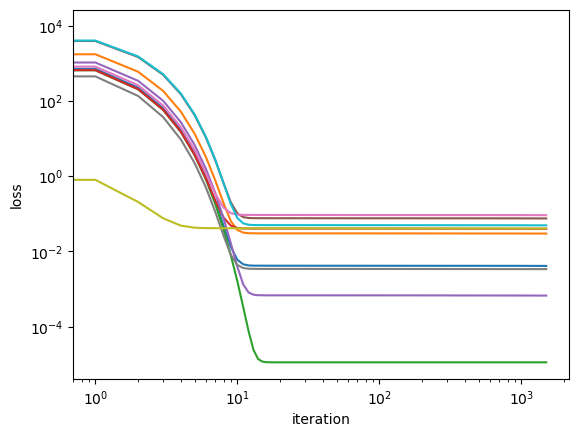
\includegraphics[scale=0.40]{loss-vs-iteration-father-away.png}
		\label{subfig:convergence-loss-father-away}
	\end{subfigure}
	\begin{subfigure}{.5\textwidth}
		\subcaption{$(k_{exp}/\alpha_{exp})$ $/$ $(k_{true}/\alpha_{true})$ vs. iteration}
		\centering
		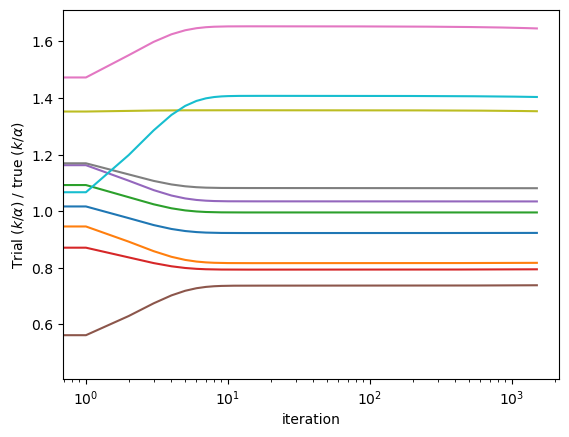
\includegraphics[scale=0.40]{k-a-ratio-father-away.png}
		\label{subfig:convergence-ratio-farther-away}
	\end{subfigure}
	\label{fig:convergence-farther-away}
\end{figure}

\subsubsection{Sampling near a fixed point}

\begin{figure}[H]
	\caption{Sampled points and associated $\ddot{q}$, for $(q_0,q_1)$ near a fixed point}
	\centering
	\includegraphics[scale=0.40]{2D-sampling-fixed-point.png}
	\label{fig:2D-sampling-fixed-point}
\end{figure}

\begin{figure}[H]
	\caption{Gradient descent performance profile, near a fixed point}
	\begin{subfigure}{.5\textwidth}
		\subcaption{Loss vs. iterations}
		\centering
		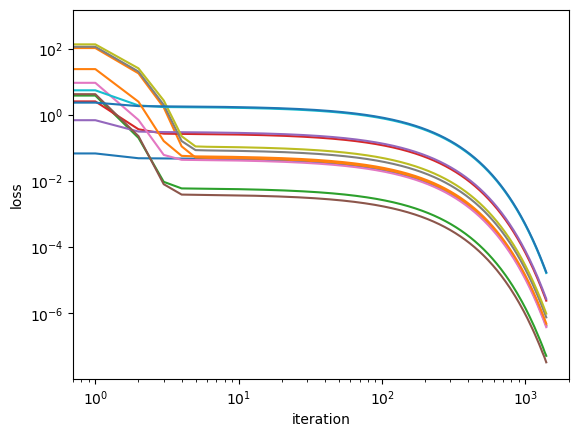
\includegraphics[scale=0.40]{loss-vs-iteration-fixed-point.png}
		\label{subfig:convergence-loss-fixed-point}
	\end{subfigure}
	\begin{subfigure}{.5\textwidth}
		\subcaption{$(k_{exp}/\alpha_{exp})$ $/$ $(k_{true}/\alpha_{true})$ vs. iteration}
		\centering
		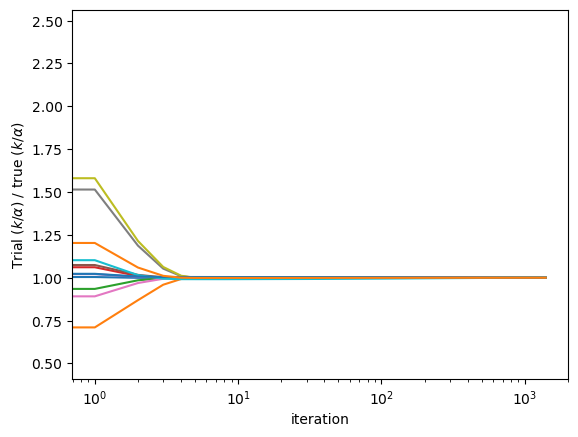
\includegraphics[scale=0.40]{k-a-ratio-fixed-point.png}
		\label{subfig:convergence-ratio-fixed-point}
	\end{subfigure}
	\label{fig:convergence-fixed-point}
\end{figure}

\subsubsection{Sampling very close to a fixed point}

\begin{figure}[H]
	\caption{Sampled points and associated $\ddot{q}$, for $(q_0,q_1)$ near a fixed point}
	\centering
	\includegraphics[scale=0.40]{2D-sampling-fixed-point-close.png}
	\label{fig:2D-sampling-fixed-point-close}
\end{figure}

\begin{figure}[H]
	\caption{Comparison of sampling near a fixed point for a large range of sampling area sizes}
	\begin{subfigure}{.5\textwidth}
		\subcaption{Box width = $0.1$}
		\centering
		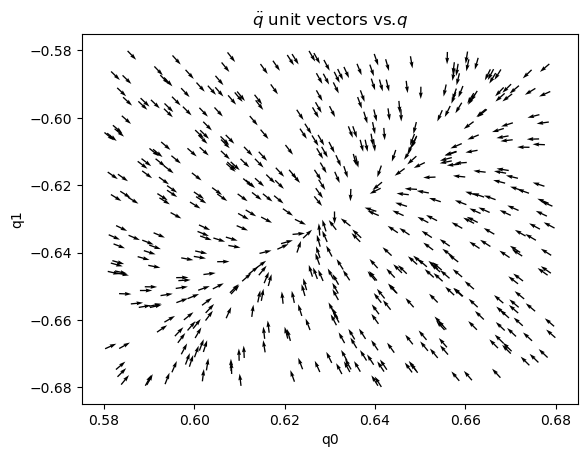
\includegraphics[scale=0.40]{2d-sampling-fixed-point-partial.png}
		\label{subfig:sampling-fixed-point}
	\end{subfigure}
	\begin{subfigure}{.5\textwidth}
		\subcaption{Box width = $0.0002$}
		\centering
		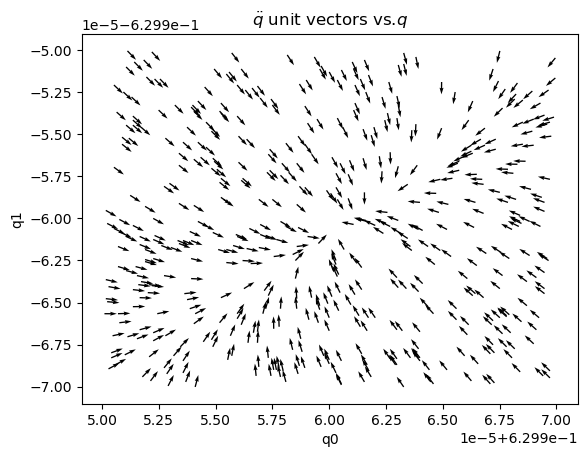
\includegraphics[scale=0.40]{2d-sampling-fixed-point-close-partial.png}
		\label{subfig:sampling-fixed-point-close}
	\end{subfigure}
	\label{fig:sampling-fixed-point}
\end{figure}

\subsection{Polynomial Lagrangian}

\begin{figure}[H]
	\caption{Training run 1: Loss vs. iteration}
	\centering
	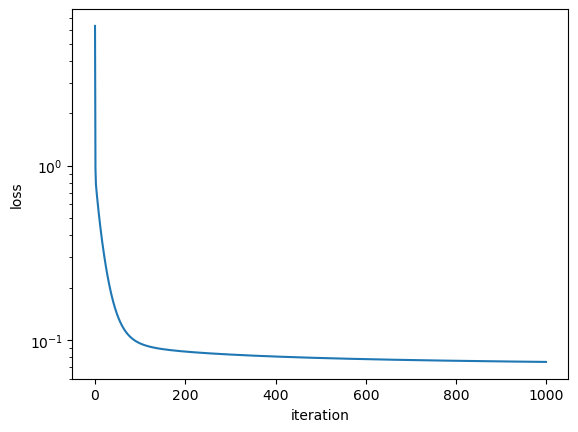
\includegraphics[scale=0.60]{poly-loss-training-1.png}
	\label{fig:poly-loss-training-1}
\end{figure}

\begin{figure}[H]
	\caption{Training run 2: Loss vs. iteration}
	\centering
	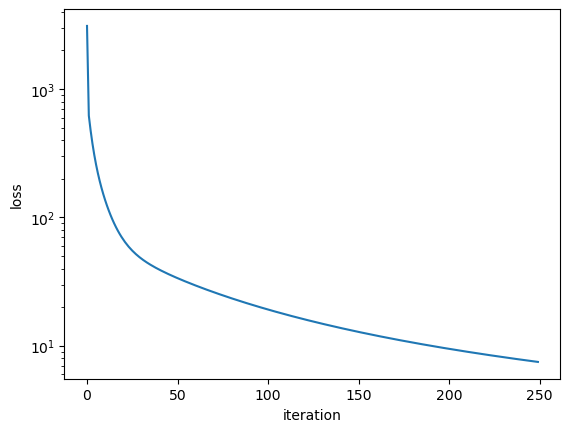
\includegraphics[scale=0.60]{poly-loss-training-2.png}
	\label{fig:poly-loss-training-2}
\end{figure}

\begin{figure}[H]
	\caption{Training run 3 (narrow sampling window): Loss vs. iteration}
	\centering
	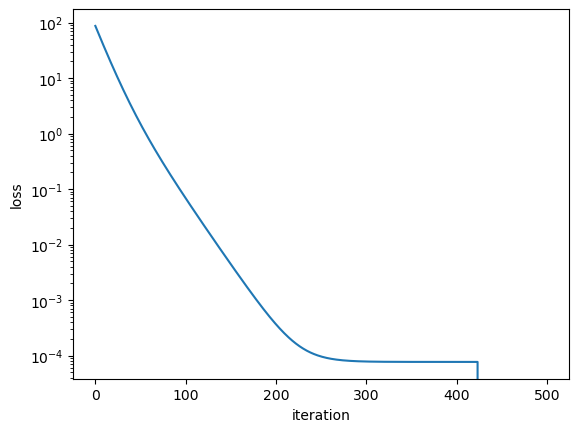
\includegraphics[scale=0.60]{poly-loss-training-3.png}
	\label{fig:poly-loss-training-3}
\end{figure}




\end{appendices}



\newpage
\begin{appendices}
	\section{Bibliography}
	\printbibliography
\end{appendices}

\end{document}